\section{Arquitectura de la red distribuida}
%\subsection{Administrar pagos admisión}
%\subsection{Administrar pagos admisión}
Desarrollo de un software que permita la implementación de un ambiente de Big Data de manera distribuida para realizar análisis
de datos aplicando diversas técnicas de minería de datos como son: aprendizaje de máquina (machine learning), como reglas de
asociación y árboles de decisión mismos que favorecen de una u otra manera a la toma de decisiones de forma práctica y sin
demasiadas complicaciones, a las empresas. El siguiente diagrama muestra la arquitectura prevista del sistema:
\\
\begin{figure}[!htbp]
	\hypertarget{fig:cap1}{\hspace{1pt}}
	\begin{center}
		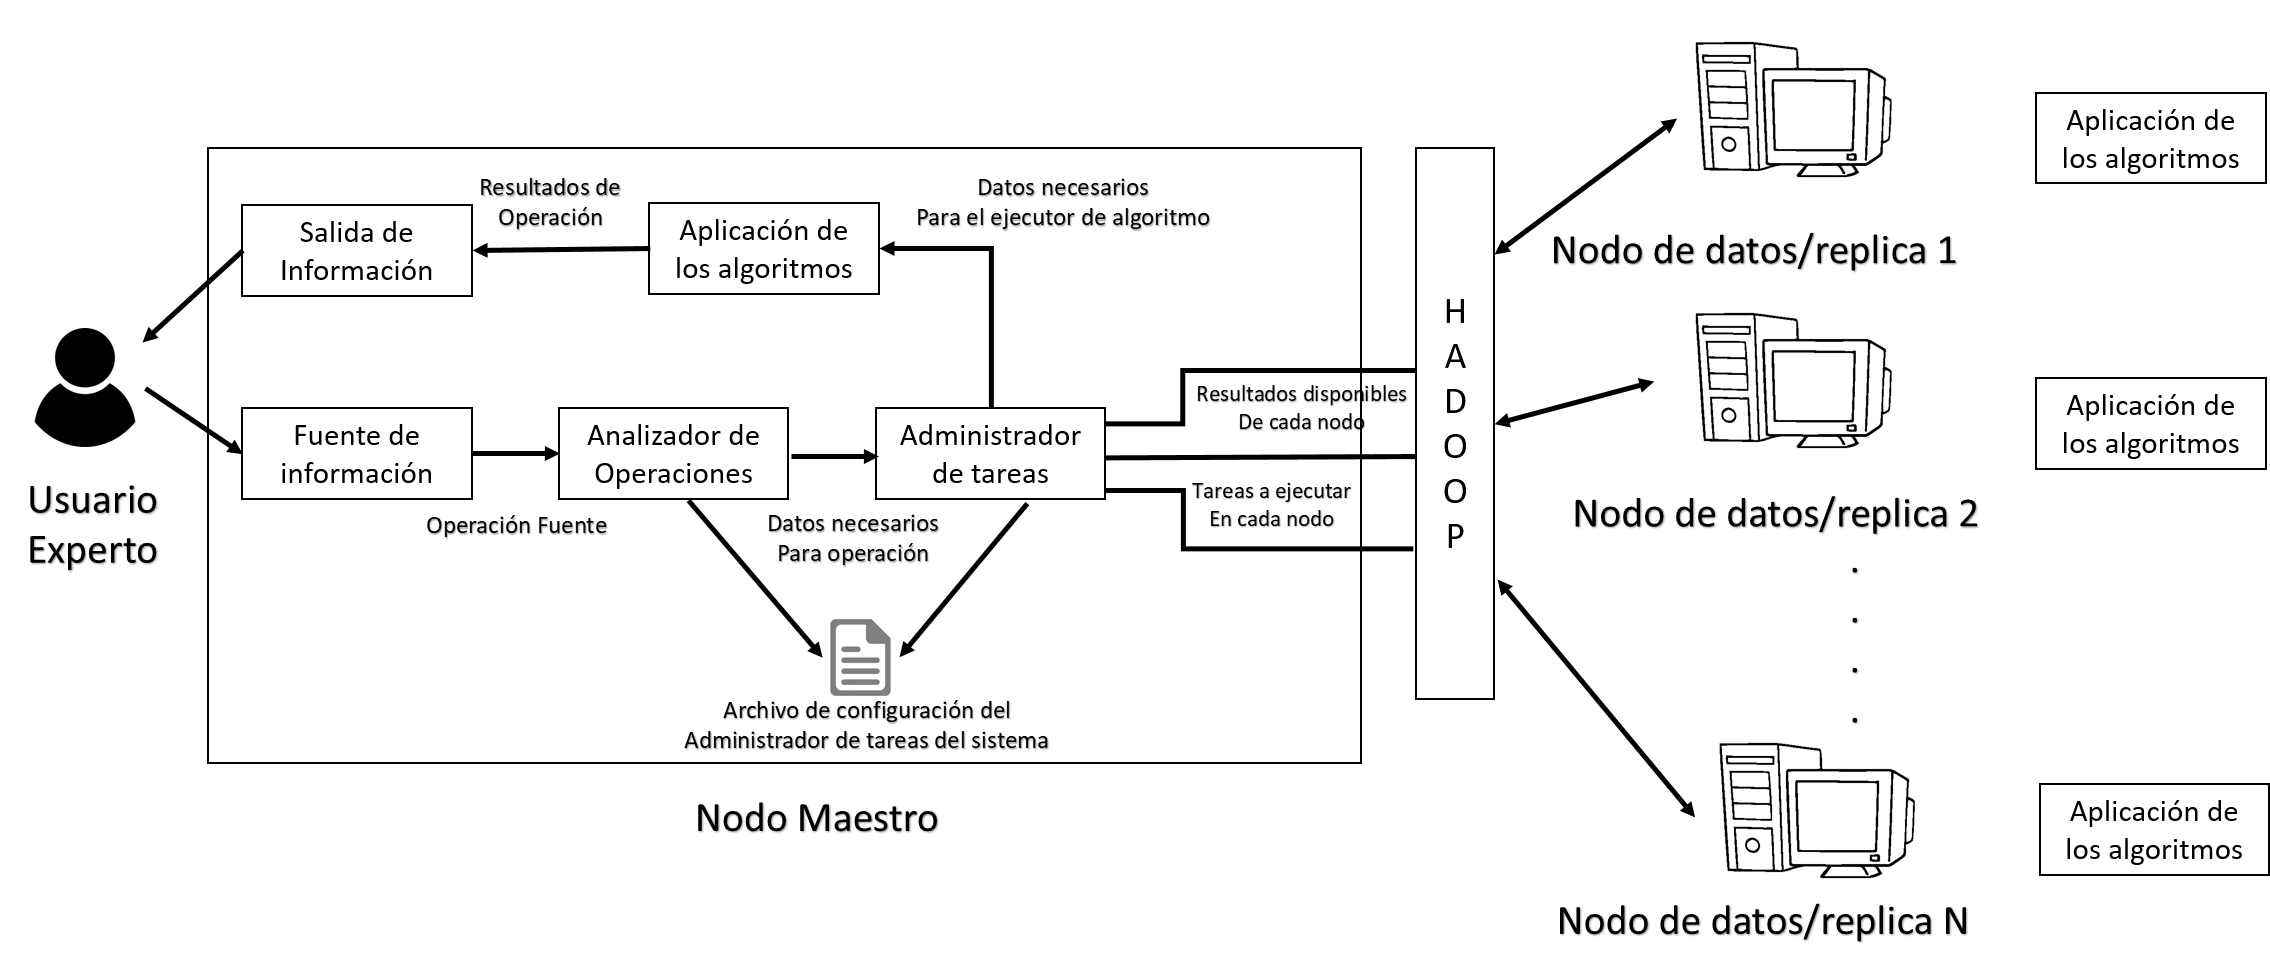
\includegraphics[height=0.3\textheight]{capitulo1/images/im1.png}
		\caption{Arquitectura de la red distribuida}
		\label{fig:cap1}
	\end{center}
\end{figure}
Con esta arquitectura será posible adaptar el Framework a diversos casos de estudio relacionados a datos de ingresos y egresos
económicos para diferentes empresas , modificando únicamente archivos que serán destinados para la configuración de dichos
casos de estudio. Esto sin tener que modificar la arquitectura del sistema ni entender su funcionamiento interno. Será posible
mantener muy bien separados los bloques de código que realizan cada actividad en el sistema para que en caso de algún fallo sea
más fácil detectar en dónde está ocurriendo.
\\
Productos esperados:
\\
\begin{enumerate}
	\item Framework funcional para el manejo de Big Data en grandes cantidades de datos. (Implementación, Código Fuente)
	\item Caso de prueba funcional implementado en el Framework
	\item Manual Técnico
	\item Manual de Usuario.
\end{enumerate}
